\section{State Of The Art Readout-Systems}

This section describes commercially available real-time oscilloscopes, as well as the \gls{kapture} system, which is in use at \gls{kara} for \gls{thz} diagnostics. Understanding the architecture of the latter will help for the development of the new system, as the basic concept of \gls{kapture} is reused there.
\subsection*{Real-Time Oscilloscope}
TODO: Overview over the current commercially available oscilloscopes.
\begin{itemize}
	\item KeySight Infiniium MXR-Series Real-Time Oscilloscopes
	\item Rohde\&Schwarz DPO70000SX
	\item LeCroy LabMaster 10-100Zi
\end{itemize}

\subsection*{\gls{kapture}}
\Gls{kapture} is a fast readout system developed at the \Gls{ipe} for \Gls{thz} diagnostics at \gls{kara}. It is designed to digitize the pulses generated by \Gls{thz} detectors at each revolution, only sampling the pulse shapes without the "empty" signal in between. The system is able to sample pulses with a \gls{fwhm} between a few tens to a hundred picoseconds with a minimal sample time of \SI{3}{\pico \second}. \cite{caselleKAP}

\subsubsection*{General Architecture}
The system consists of two parts: the sampling front-end card and a \gls{fpga} readout card. In \autoref{fig:thz_chain} the setup for \gls{thz} radiation measurements with \gls{kapture} is shown. 

The incoming radiation is fed into a detector, which converts the incident photons into an electrical signal. This signal is then amplified in a wide-band \gls{lna}. The latter splits the detector signal into four identical signals, which are then propagated to the sampling front-end card. The card consists of four parallel sampling channels with adjustable sample time, each containing a \gls{tha} and an ADC. This card is connected to a read-out card, which has two tasks: programming the components on the front-end card (\gls{fpga}-part) and sending the acquired data to a PC/\gls{daq} system. \cite{caselle2014}

\begin{figure}[tbh]
	\centering
	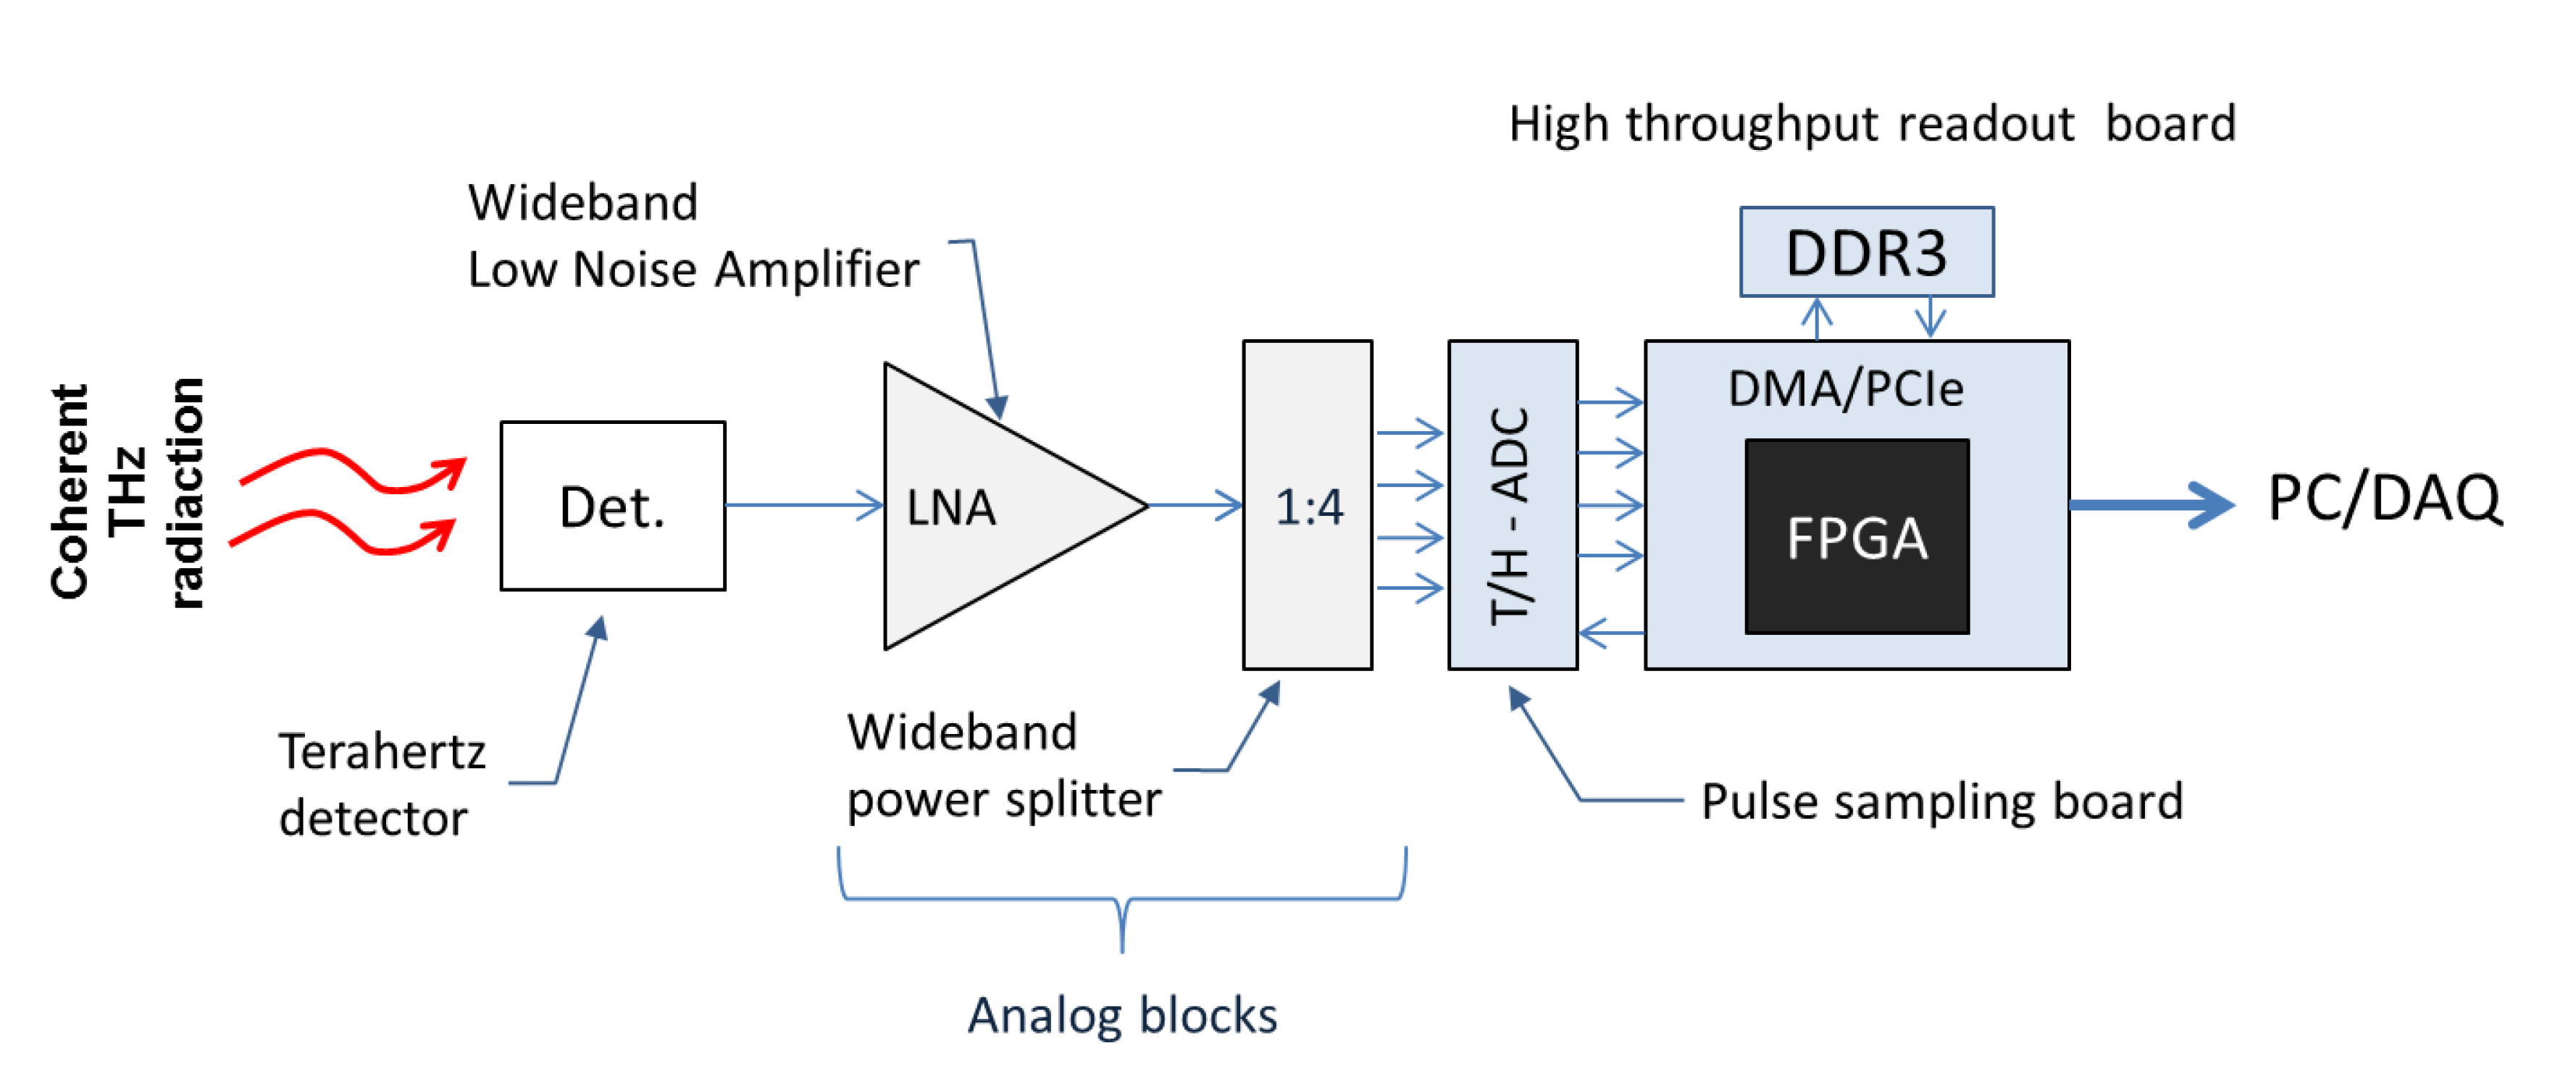
\includegraphics[width = \textwidth]{chap/03-currentStat/img/thz_chain}
	\caption[THz measurement with KAPTURE]{\gls{thz} radiation measurement setup with \gls{kapture}(cf. \cite{caselle2014})}
	\label{fig:thz_chain}
\end{figure}

\paragraph{Analog Front-End}
Due to the high bandwidth nature of the detector signal, the analog front-end of the system has to be wideband as well to be able to sample the signal with picosecond resolution. 

The used \gls{lna} is based on a commercial GaAs \gls{mmic} which operates from DC to \SI{50}{\giga \hertz}. It is needed to compensate the insertion loss\footnote{\textit{Insertion loss} is the loss of signal power which occurs, when a signal passes through a component.} due to the following power splitter. %todo maybe more info, ask michele

Classical power-splitters are not intrinsically wideband (\cite{caselle2014}). For that reason, an wideband power-splitter was developed at \gls{ipe} which fulfills the bandwidth requirements. The designed power-splitter works up to \SI{100}{\giga \hertz} with an insertion loss of \SI{8}{\decibel} and a return loss\footnote{\textit{Return loss} is the loss of signal power due to reflection by a discontinuity in the transmission line.} of about \SI{20}{\decibel} at \SI{50}{\giga \hertz}.\cite{caselle2014}

\paragraph{Sampling Board}
The general structure of the board with the power splitter is shown in \autoref{fig:kapture}. 
\begin{figure}[tbh]
	\centering
	\includegraphics[width = \textwidth]{chap/03-currentStat/img/kapture.tikz}
	\caption[General architecture of the KAPTURE system]{General architecture of the KAPTURE front-end sampling card (cf. \cite[p.2]{caselleKAP})}
	\label{fig:kapture}
\end{figure}

Four identical signals from the power-splitter are fed into four channels, consisting of a respective \gls{tha} unit and a 12-bit \gls{adc} sampling at \SI{500}{\mega\sample\per\second}. The sampling time of each unit can be adjusted individually with a delay chip with a resolution of \SI{3}{\pico \second} (maximal delay range: \SI{100}{\pico \second}). The delay chips are programmed with the \gls{fpga} on the readout card.
The clock signal is provided by \gls{kara}, which is cleared from jitter by a \gls{pll}. This ensures the synchronization of the \glspl{adc} with the \gls{rf} system. The cleaned clock signal is distributed to the delay chips via fan-out buffer. \cite{caselleKAP}
In this way, the pulse can be "locally sampled" by adjusting the different delay with a maximum rate of 330 GS/s possible. 
A simplified representation of the local sampling of the signal is shown in \autoref{fig:detector_signal}.
\begin{figure}[tbh]
	\centering
	\includegraphics[width = \textwidth, height=0.4\textwidth]{chap/03-currentStat/img/detector_signal.tikz}
	\caption{Signal and sampled points $S_1$ to $S_4$}
	\label{fig:detector_signal}
\end{figure}

\autoref{fig:kapturesys} shows a photo of the system setup at \gls{kara}
\begin{figure}[tbh]
	\centering
	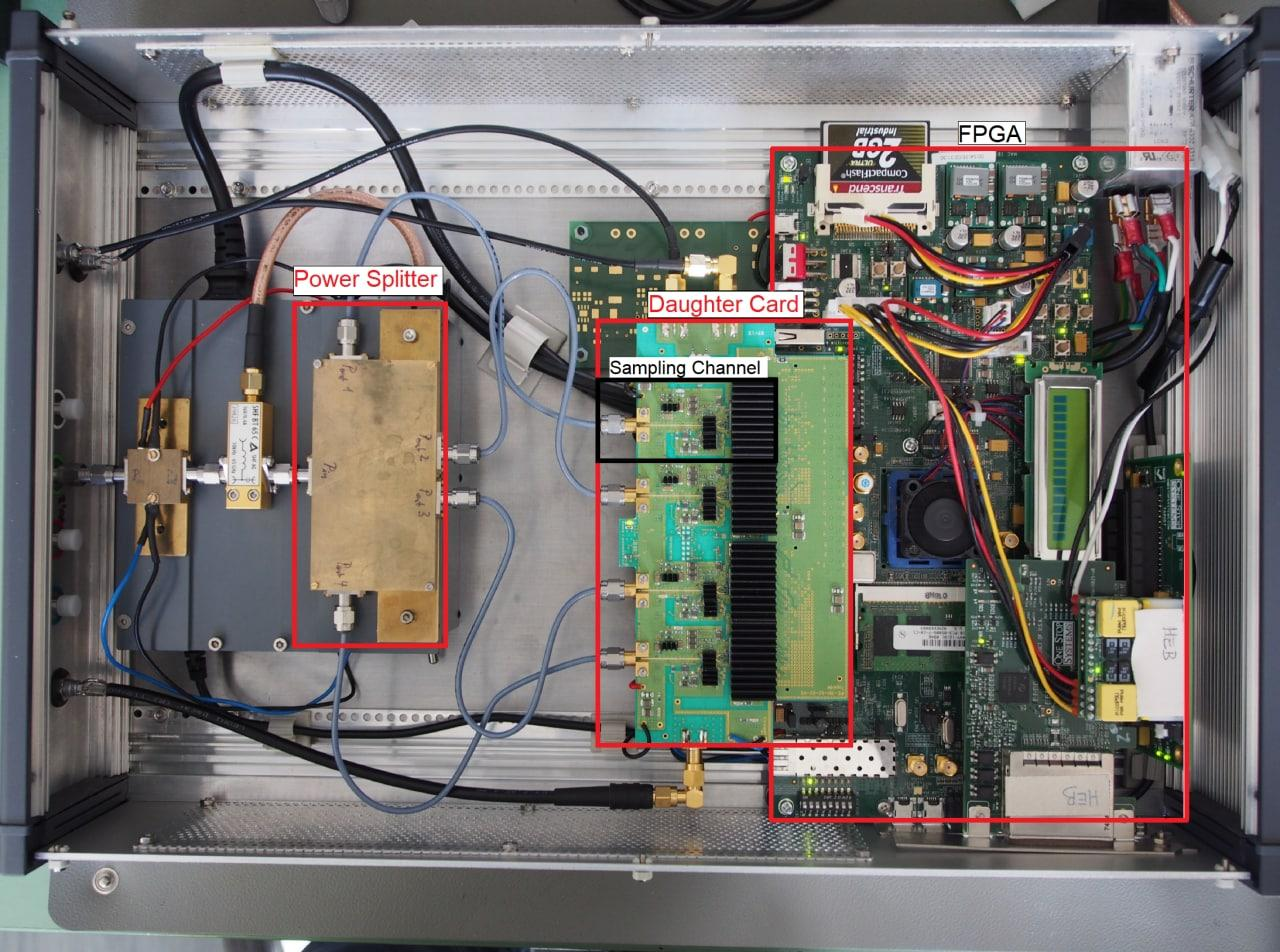
\includegraphics[width = \textwidth]{chap/03-currentStat/img/kapture_sys}
	\caption[Photo of KAPTURE system]{Photo of KAPTURE with highlighted main components. \cite[p.~61]{brosi}}
	\label{fig:kapturesys}
\end{figure}
%todo  re-label

\paragraph{PC/Data-Acquisition System}
In order to keep a continuous data acquisition the necessary bandwidth is 
\begin{equation}
	12 \text{bits} \cdot 4 \, \text{samples} \cdot \SI{500}{\mega \hertz} = 24 \text{Gb/s}
\end{equation}
To ensure high data throughput, the readout board is based on a bus master \gls{dma} architecture which is connected to \gls{pcie} end-point logic. This ensures a throughput of up to 2 GByte/s. To store the data temporary before it is sent to the \gls{daq} system, a large \gls{ddr}3 memory device is used, as seen in \autoref{fig:kapture}. \cite{caselleKAP}

TODO: briefly explain newer DAQ system with GPU architecture

Briefly mention KAPTURE-2 also? 


\begin{figure}[tbh]
	\centering
	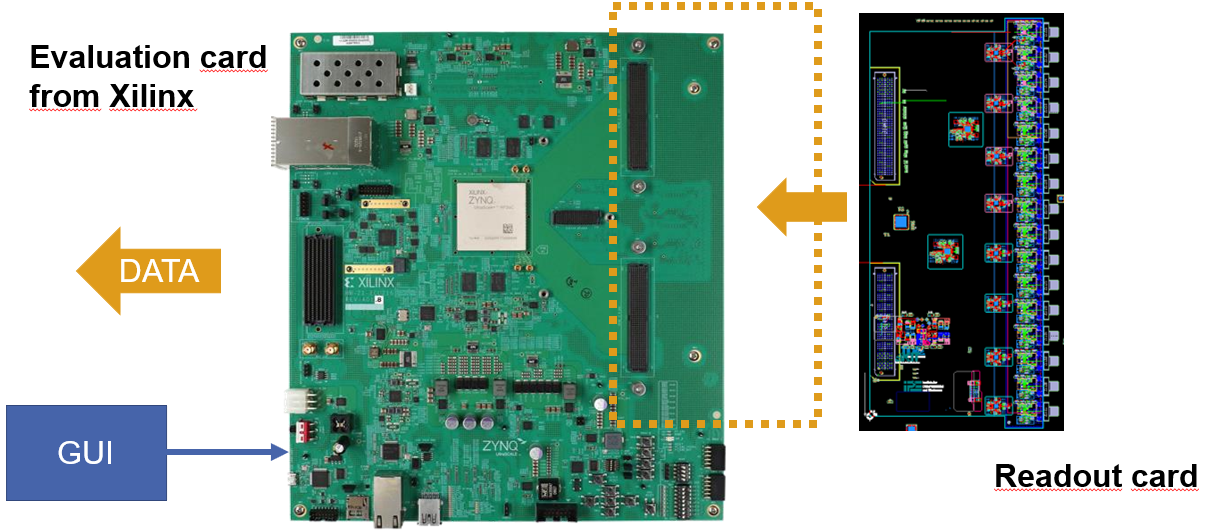
\includegraphics[width = \textwidth]{chap/04-work/img/concept_theresa}
	\caption{General concept of the new readout system}
	\label{fig:concept_theresa}
\end{figure}
\textbf{TODO:} Picture of the WHOLE system, i.e. with the optical front end + power splitter + theresa + zcu216

\section{New System}
\subsection*{Optical Part}
"femtosecond Ytterbium-doped fiber laser (Orange) from MENLO GmbH. The emitted pulses have a spectral bandwidth of 50 nm, and the total
output average power is 40 mW. The repetition rate is chosen at 88 MHz, which corresponds to 1/4 th of
the RF frequency of Synchrotron SOLEIL and 104 times the electron revolution frequency."

\paragraph{Photodetector}
The detection and subtraction between the two stretched signals is performed using a amplified balanced photodetector (photoreceiver) from Discovery Semiconductors, with 20 GHz bandwidth and 2800 V/W gain (specified at 1500 nm).

\subsection*{Front-End Card}
\autoref{fig:theresa_scheme} shows the general schema of the sampling system, reduced to four channels for presentation purposes.
\begin{figure}[H]
	\centering
	\includegraphics[width = \textwidth]{chap/04-work/img/theresa_scheme.tikz}
	\caption[General architecture of THERESA]{General architecture of THERESA with power splitter and \glspl{adc}. For presentation purposes only four of the sixteen channels are shown.}
	\label{fig:theresa_scheme}
\end{figure}

\subsubsection*{Time Interleaving}\label{sssec:time-interleaving}
%TODO explain that we plan to use time interleaving in order to increase the sampling rate
In order to increase the sampling rate, the so called time-interleaving technique is used. In this section, first basic theory about this technique is given. Then, the implementation in the new system is described.

\paragraph{Theory}
In the \textit{Time Interleaving} technique multiple \glspl{adc} are used in such way, that allows to sample data at a faster rate, than the respective sample rate of each individual \gls{adc}. The principle is based on time-multiplexing an array of $M$ identical \glspl{adc} (see \autoref{fig:adc_interleaving}), each sampling at $f_c = f_s/M$ individually. This means, the \glspl{adc} are clocked in such a way, that they start their respective conversion cycle shortly one after another. At time $t_0$ the first \gls{adc} starts converting the input signal $V_i(t_0)$, after a time delay $\Delta t_i$ the second starts converting the signal $V_i(t_0 + t_i)$, the third converts $V_i(t_0 + 2t_i)$ and so on. After the $M$-th \gls{adc} has sampled the signal $V_i(t_0 + (M-1)t_i)$, the whole cycle starts anew with the first converter. \cite{mangrob}
\begin{figure}[tbh]
	\centering
	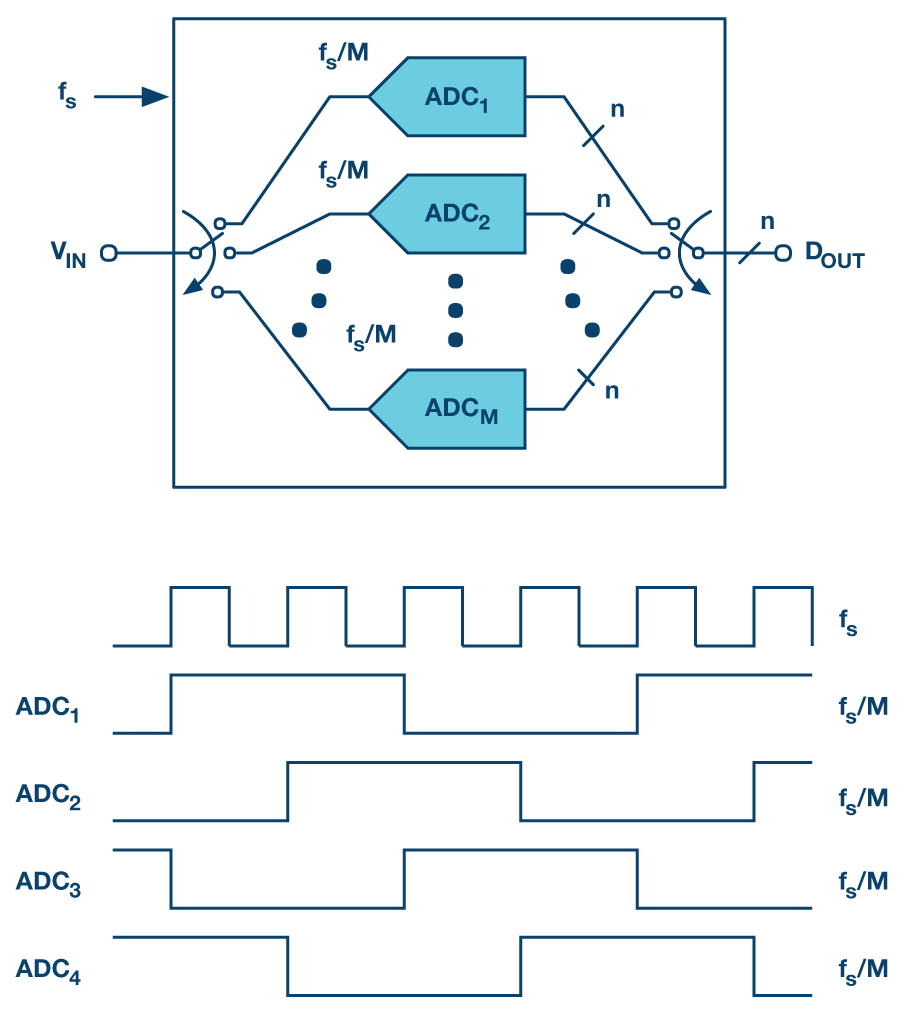
\includegraphics[width = \textwidth]{chap/02-theory/img/adc_inter}
	\caption[Time Interleaving]{Placeholder: An array of $M$ time interleaved $N$-bit \glspl{adc} with example of clocking scheme for the case of $M$ = 4 \cite{mangrob}}
	\label{fig:adc_interleaving}
\end{figure}
%todo to tikz
\paragraph{Challenges}
Spurs appear in the spectrum. There are several reasons for this.

First reason is the \textit{offset mismatch} between den \glspl{adc}. Each \gls{adc} has an DC offset value. Considering as example an interleaving structure with two \glspl{adc} and a constant input voltage: when the samples are acquired back and forth between the two \glspl{adc}, the resulting output will switch back and forth between two levels due to the different offset levels. This output switches at the frequency $f_s/2$ and therefore introduces an additional frequency component in the spectrum (see \autoref{fig:offset_mm}). The magnitude of the spur depends on the offset difference between the \glspl{adc}. \cite{Harris2019}

\begin{figure}[tbh]
	\centering
	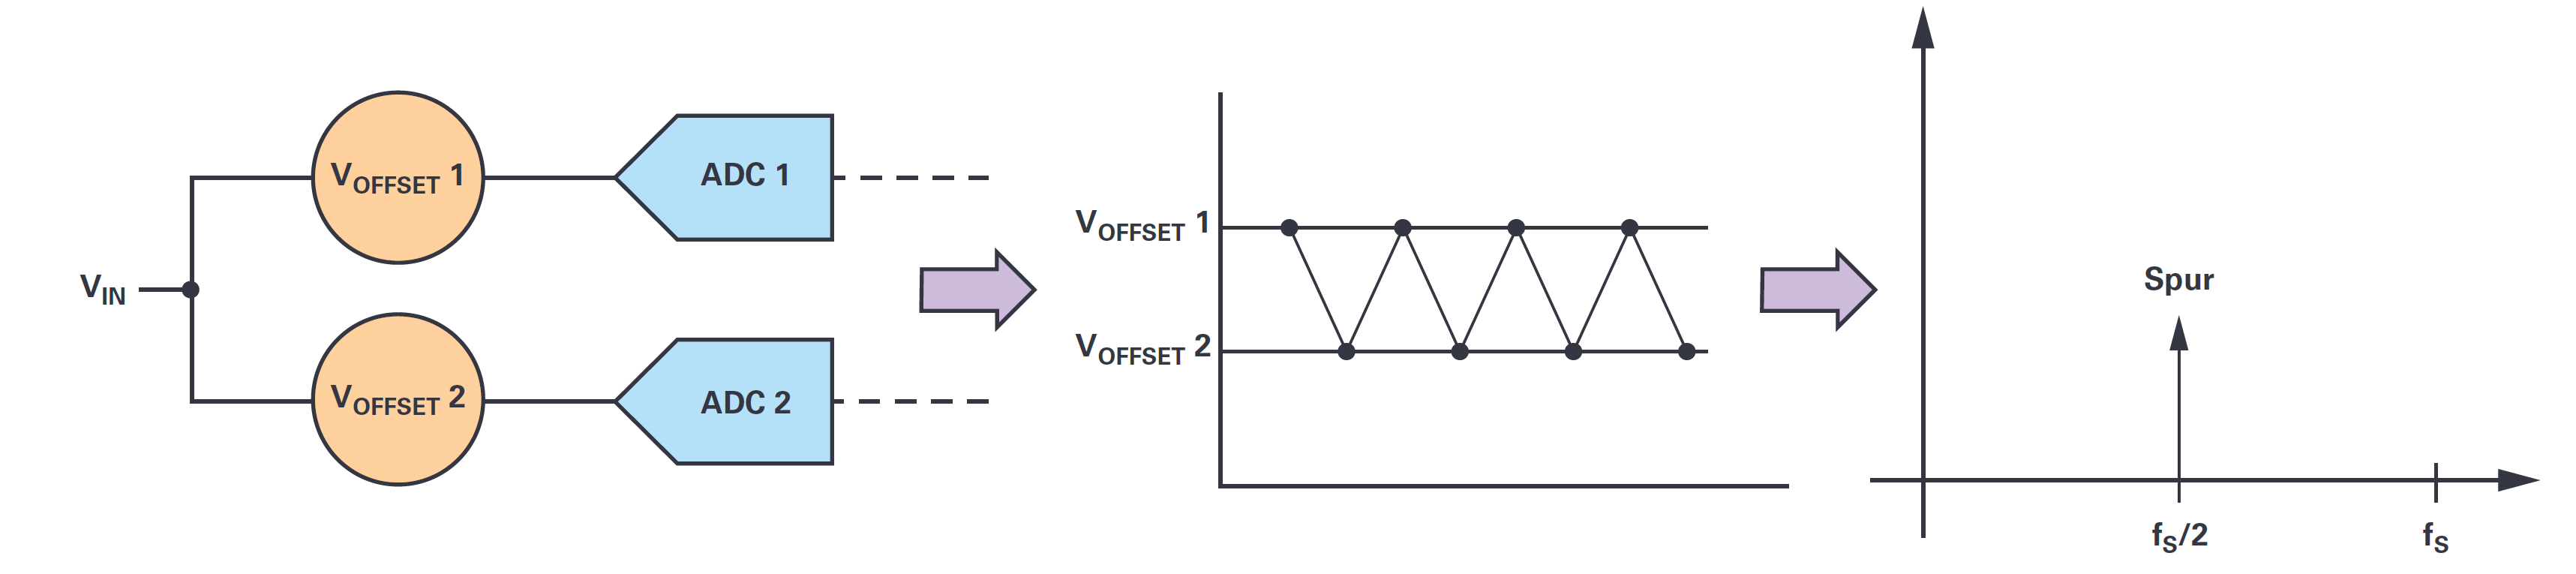
\includegraphics[width = \textwidth]{chap/02-theory/img/offset_mm}
	\caption{Placeholder: Offset-Mismatch in Interleaving \cite{Harris2019}}
	\label{fig:offset_mm}
\end{figure}

Besides of the offset also the gain of the converters can be mismatched. This \textit{gain mismatch} has a frequency component to it, which in case of an input signal of the frequency $f_{\text{in}}$ results in a spur at $f_s/2 \pm f_{\text{in}}$ (see \autoref{fig:gain_mm}). \cite{Harris2019}

\begin{figure}[tbh]
	\centering
	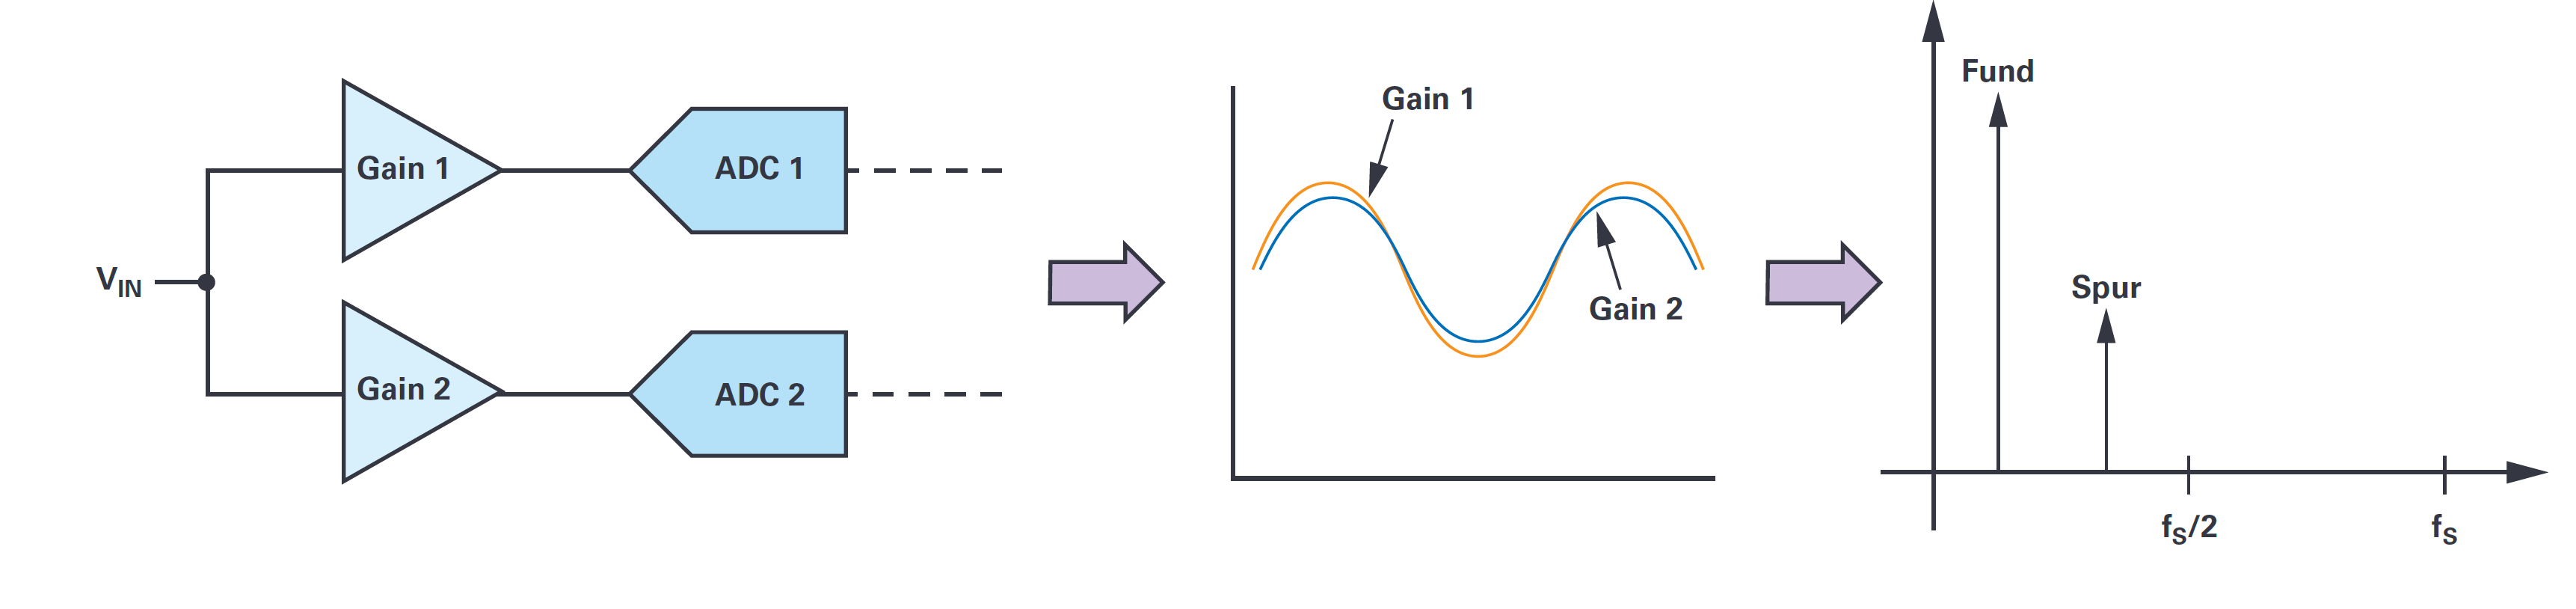
\includegraphics[width = \textwidth]{chap/02-theory/img/gain_mm}
	\caption{Placeholder: Gain-Mismatch in Interleaving \cite{Harris2019}}
	\label{fig:gain_mm}
\end{figure}

In the time domain, \textit{timing mismatch} due to group delay in the analog circuitry of the \gls{adc} and clock skew\footnote{Difference in arrival time of the clock signal at different components.} can occur. The group delay in analog circuitry can vary between the converters. Furthermore, the clock skew has on the one hand an aperture uncertainty component at each of the \glspl{adc} and on the other hand a component related to the accuracy of the clock phases, which are input to each converter. \cite{Harris2019} This mismatch also produces a spur at $f_s/2 \pm f_{\text{in}}$ (see \autoref{fig:timing_mm}).

\begin{figure}[tbh]
	\centering
	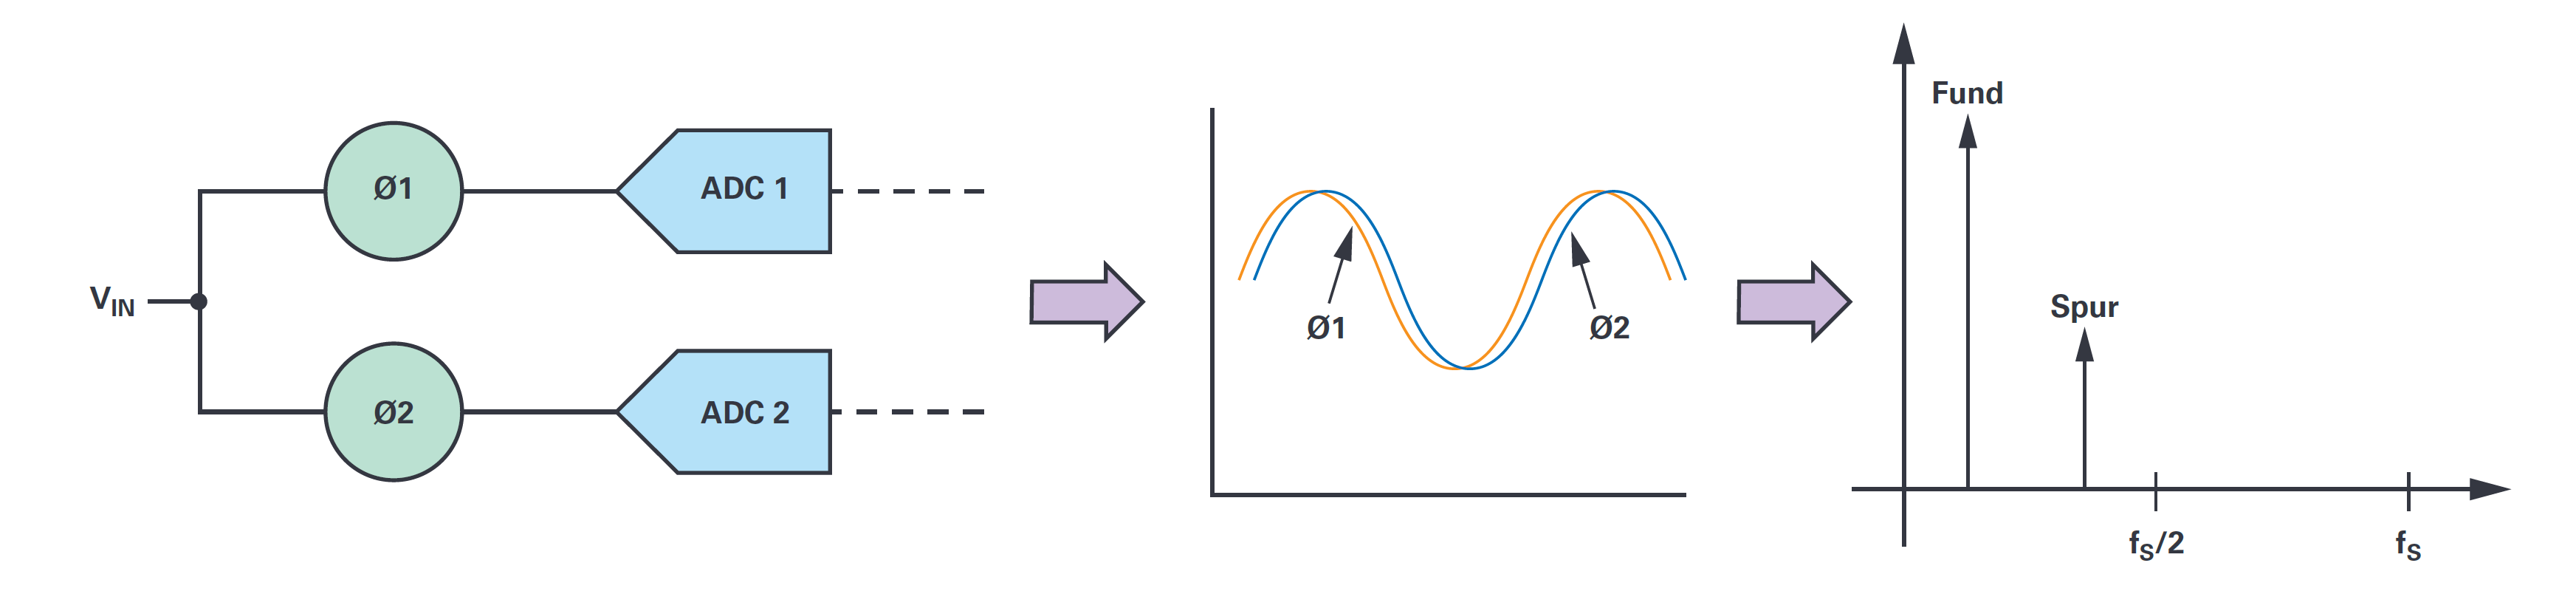
\includegraphics[width = \textwidth]{chap/02-theory/img/timing_mm}
	\caption{Placeholder: Timing-Mismatch in Interleaving \cite{Harris2019}}
	\label{fig:timing_mm}
\end{figure}

The last possible mismatch is the \textit{bandwidth mismatch}, which contains both gain and phase/frequency component (see \autoref{fig:bandwidth_mm}). Due to bandwidth mismatch, different gain values at different frequencies can be seen. An additional timing component causes different delays for signals at different frequencies through each \gls{adc}. Just like gain and timing mismatch, the bandwidth mismatch causes a spur at $f_s/2 \pm f_{\text{in}}$.
\begin{figure}[tbh]
	\centering
	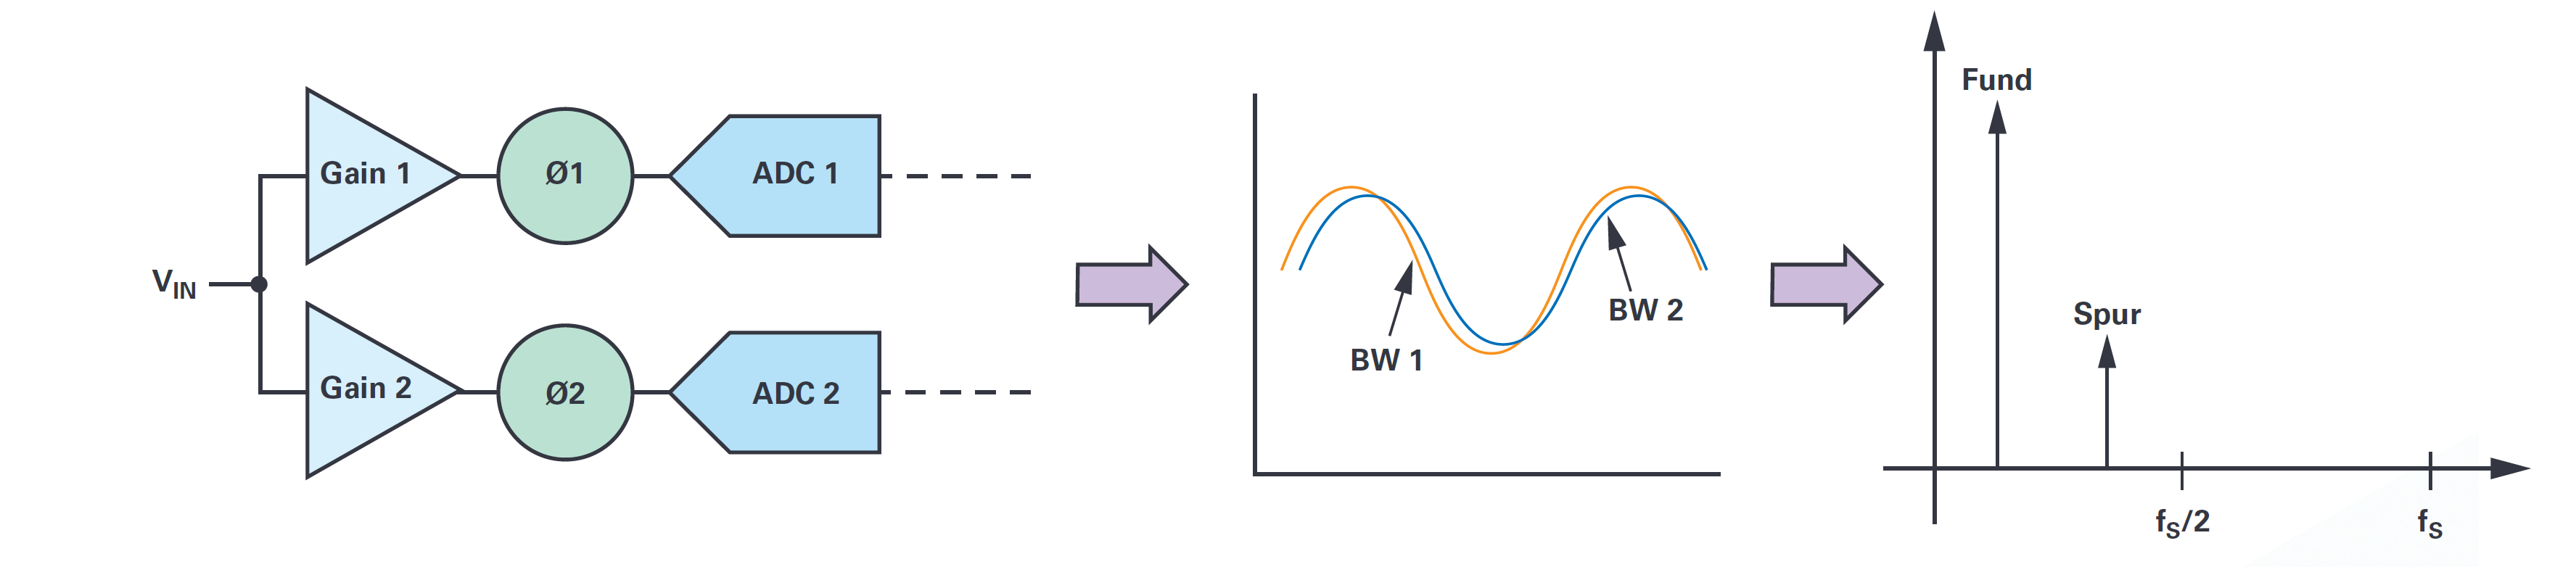
\includegraphics[width = \textwidth]{chap/02-theory/img/bandwidth_mm}
	\caption{Placeholder: Timing-Mismatch in Interleaving \cite{Harris2019}}
	\label{fig:bandwidth_mm}
\end{figure}

\paragraph{Implementation}\label{ssec:interl_impl}
The delay step size must be small enough, such that the \gls{adc} interleaving technique \autoref{sssec:time-interleaving} can be implemented.
The \glspl{adc} on the read-out card sample at a maximal sample rate of \SI{2.5}{\giga \sample \per \second}, meaning during the time
\begin{equation}
	t_s = \frac{1}{\SI{2.5}{\giga \sample \per \second}} = \SI{400}{\pico \second}
\end{equation}
all 16 \glspl{adc} have to be clocked one time.
This means, a delay step can not be greater than $\nicefrac{\SI{400}{\pico\second}}{16} = \SI{25}{\pico\second}$.

Clock to THA: \SI{2}{\GHz}
$\rightarrow$ Step size for delay:
\begin{equation}
	\frac{\SI{1}{\nano \second}}{16 \, \text{channels}} = \SI{62.5}{\pico \second}
\end{equation}

Aperture delay, jitter, need to be taken into account to determine the max. sampling frequency.

\begin{sidewaysfigure}[tbh]
	\centering
	\tikzexternaldisable
	\includegraphics[width = 0.8\textwidth]{chap/04-work/img/interl_timing}
	\tikzexternalenable
	\caption[Track-And-Hold Timing diagram]{\gls{tha} Timing diagram. Shows the clocking of the \gls{tha} (HIGH = hold mode, LOW = track mode). Dashed line represents the sampling of the \gls{adc}.}
	\label{fig:THA}
\end{sidewaysfigure}

The necessary step size for the delay chips, when using 16 ADC@\SI{2}{\giga \sample \per \second} in time-interleaving mode, is: $\frac{\SI{2}{\giga \sample \per \second}}{16} = \SI{31}{\pico \second}$
However, providing individual clocks to the ADCs is not possible on the ZCU216 card. ADCs are grouped together into tiles, each tile containing four converters. One single reference clock signal is propagated to all tiles. Sampling clock is adjusted at each tile individually, however this clocking signal is the same for all of the four converters in the tile. Normally, only one reference clock can be provided. Analyzing the schematic of the ZCU216 board revealed however, that there are pins leading to the FPGA banks (224 to 227), labeled as clocks for the individual tiles. Two of the clocks are not connected (224 and 227). 225 is provided via SMA cable, the other comes from the LPAM clock connector. 

\subsection*{Readout Card}
\textbf{TODO}
\subsubsection*{Selection Of The Card}\label{sec:selection}
When selecting the Readout Card, following criteria need to be considered:
\begin{itemize}
	\item Integrated \glspl{adc}
	\item Number, resolution and bandwidth of \glspl{adc}
	\item Peripheral connections
	\item Flexibility/Customization
	\item Suitable connectivity for high-data-throughput
\end{itemize}

Footprint of using all discrete components is, as one can imagine, higher, than if you integrate all the parts into on \gls{ic}. Not only the footprint is a concern, but also the number of connections. ADCs with high resolution, a high number of ADCs therefore explodes the necessary amount of connections. 
\begin{figure}[tbh]
	\centering
	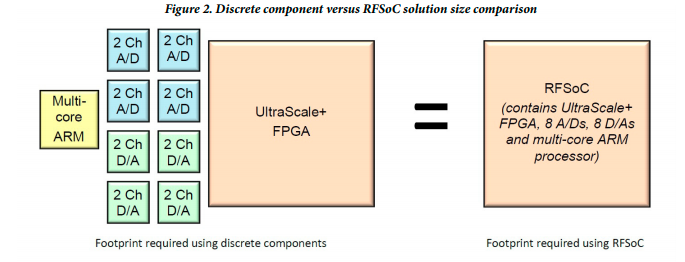
\includegraphics[width = \textwidth]{chap/04-work/img/footprint}
	\caption{Placeholder: Discrete vs IC}
	\label{fig:footprint}
\end{figure}
High number of ADCs also means 
